\chapter{Two Days, Two Devices}\label{ch:B1}

This chapter answers \textbf{B1} of Part B (10 marks). Both teammates captured six ten-minute
windows each, spread over two days and three time bands, and this chapter compares what those
windows show about round-trip time and about what the machines were doing when we were not
looking.

Team: 2024CS10300 (Windows 11, MediaTek Wi-Fi 6) and 2024CS10582 (Ubuntu, Intel \texttt{wlo1}).
The RTT figures come from the per-window \texttt{netlab\_gen} logs, 20 ICMP echoes per target per
window. All twelve windows are complete.

\section{Caveats, stated once and relied on throughout}

\textbf{(a) Address family.} T2 and T5 are not strict cross-device absolute-RTT comparisons.
2024CS10582 has IPv6 and reached \texttt{www.iitd.ac.in} at \texttt{2001:df4:e000:29::212} and
\texttt{www.mit.edu} at \texttt{2600:140f:5:2093::255e}; 2024CS10300 is IPv4-only and reached
\texttt{10.10.211.212} and \texttt{23.15.150.186}. In D2W3 this produces a 95.0\,ms vs 8.55\,ms
median split on T5: the same hostname, two different Akamai nodes, and no useful comparison
between them. \textbf{T3 (8.8.8.8) is IPv4 on both hosts and is the only clean cross-device
comparison}, which is why the analysis below leans on it.

\textbf{(b) Resolution.} Windows \texttt{ping} reports whole milliseconds, Linux two decimals. A
Windows median of ``48'' means 47.5--48.5.

\textbf{(c) p95 from 20 samples is the second-largest value.} It moves on one or two packets. We
treat large p95 excursions as observations, not as distribution shifts.

\textbf{(d) Per-hop traceroute times are unreliable on this path.} See
Section~\ref{sec:b1hopcaveat}.

\section{Data}

\begin{table}[H]
\centering
\caption{T2: \texttt{www.iitd.ac.in} (on campus). Median and p95 RTT in ms, 20 echoes per
window per device.}
\label{tab:b1t2}
\footnotesize
\begin{tabular}{@{}llcccc@{}}
\toprule
Window & Date & 10300 median & 10300 p95 & 10582 median & 10582 p95 \\
\midrule
D1W1 & 22-08 & 4.0 & 9.3 & 2.65 & 6.85 \\
D1W2 & 20-08 & 7.0 & 7.3 & 3.83 & 5.14 \\
D1W3 & 20-08 & 8.0 & 17.6 & 5.71 & 12.80 \\
D2W1 & 21-08 & 4.0 & 6.0 & 5.12 & 5.84 \\
D2W2 & 21-08 & 5.5 & 11.1 & 4.46 & 8.37 \\
D2W3 & 22-08 & 5.0 & 22.20 & 3.03 & 5.73 \\
\bottomrule
\end{tabular}
\end{table}

\begin{table}[H]
\centering
\caption{T3: 8.8.8.8 (off campus). Median and p95 RTT in ms. The two windows recorded on
22-08 are set in bold.}
\label{tab:b1t3}
\footnotesize
\begin{tabular}{@{}llcccc@{}}
\toprule
Window & Date & 10300 median & 10300 p95 & 10582 median & 10582 p95 \\
\midrule
D1W1 & \textbf{22-08} & \textbf{59.0} & 66.1 & \textbf{60.50} & 61.08 \\
D1W2 & 20-08 & 48.0 & 60.1 & 50.35 & 54.19 \\
D1W3 & 20-08 & 46.0 & 53.2 & 45.80 & 48.27 \\
D2W1 & 21-08 & 46.0 & 52.9 & 46.25 & 51.28 \\
D2W2 & 21-08 & 45.0 & 49.0 & 44.60 & 48.11 \\
D2W3 & \textbf{22-08} & \textbf{65.0} & 69.05 & \textbf{59.70} & 83.09 \\
\bottomrule
\end{tabular}
\end{table}

\textbf{T4} (\texttt{www.iitb.ac.in}, 103.21.124.133) returned 0 of 20 echo replies in every
window on both devices, so it carries no RTT series, the same 100\% loss Part~A reports in
Chapter~\ref{ch:Implementation}. Its traceroute consistently reached 10.10.10.1 before subsequent
probes timed out. This shows probes progressed a long way down the path but does not establish
that the destination host was reachable: a router can answer TTL-expired probes while the
destination is unreachable or filters echo. Every hop on the T4 path is RFC1918
(10.184.0.13 \ldots\ 10.10.10.1, thirteen hops), whereas the T3 path shows public addresses from
hop 9 onward; on the T4 path we never observe a packet in public address space at all.

\section{Plots}

\begin{figure}[H]
    \centering
    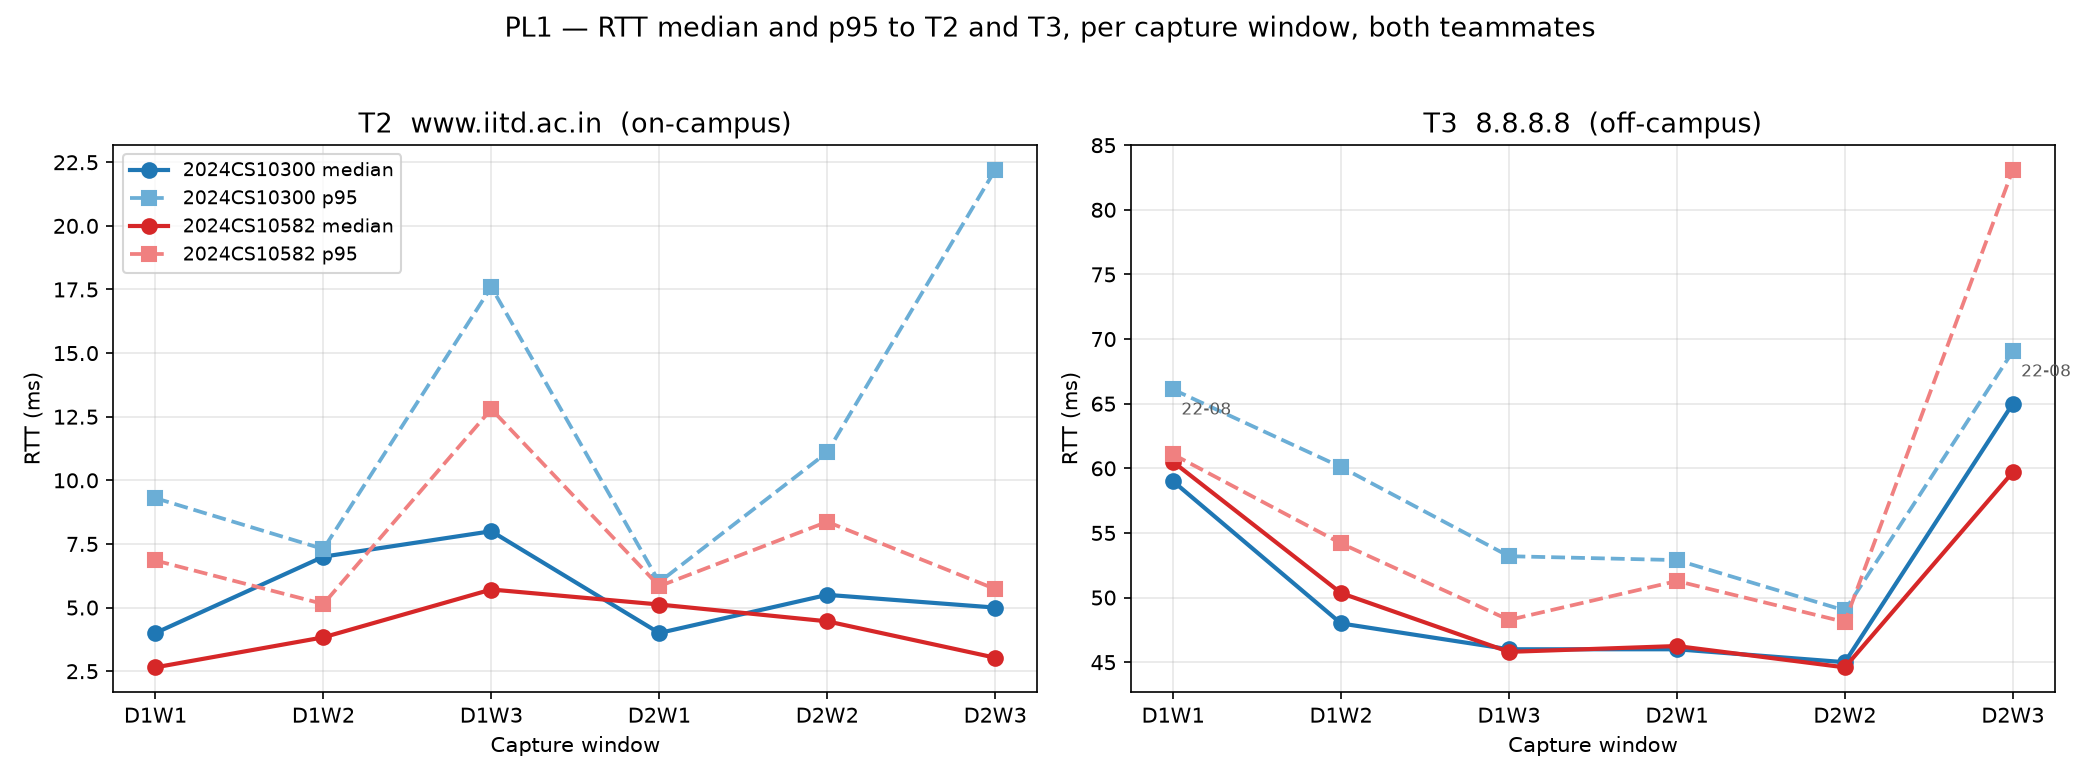
\includegraphics[width=\textwidth]{report/images/pl1_rtt_per_window.png}
    \caption[PL1: RTT median and p95 per capture window]{\textbf{PL1.} T3 RTT separates
    cleanly by calendar date, not by time of day: both windows recorded on 22-08 (D1W1, D2W3) sit
    at 59--65\,ms on both devices, while all four windows recorded on 20-08 and 21-08 sit at
    44.6--50.4\,ms. Two independent laptops moving together by $\sim$14\,ms across a date boundary
    points at the shared upstream path rather than at either machine. The T2 series shows no
    comparable structure.}
    \label{fig:pl1}
\end{figure}

\begin{figure}[H]
    \centering
    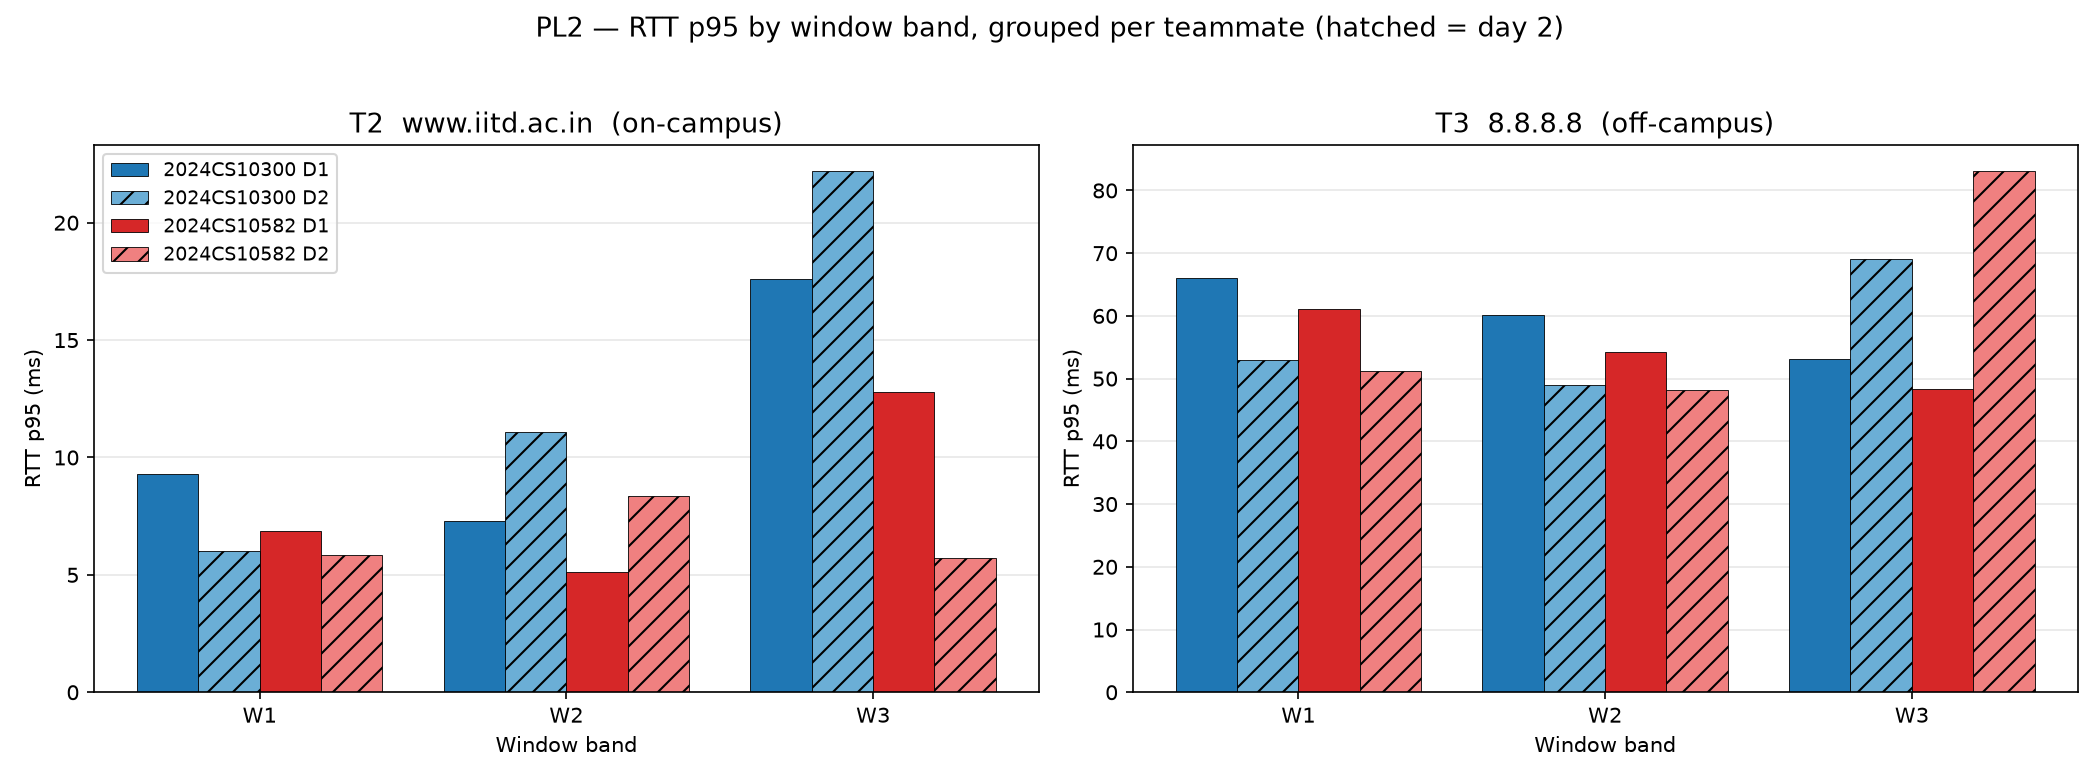
\includegraphics[width=\textwidth]{report/images/pl2_p95_by_band.png}
    \caption[PL2: RTT p95 by window band]{\textbf{PL2.} T2 p95 is largest in W3 for both
    teammates (22.20\,ms and 12.80\,ms), but the two devices peak on different days and disagree
    by a factor of four within the same evening, so the evening effect on the campus path is weak
    and inconsistent. T3 p95 shows no band structure at all; its variation follows the date,
    which is visible in PL1 and invisible here.}
    \label{fig:pl2}
\end{figure}

\section{Q1: Which window was worst for each of us? Same or different?}

\subsection{T3 (off campus): the same two windows are worst for both of us, and they share a
date}

D2W3 is the worst T3 window for both teammates (65.0\,ms median for 2024CS10300 and 59.70\,ms
for 2024CS10582), and D1W1 is second worst for both, at 59.0\,ms and 60.50\,ms. Every other
window sits between 44.6 and 50.4\,ms on both machines.

The two elevated windows are D1W1 (22-08, 09:00 IST) and D2W3 (22-08, 21:00 IST). The four
normal windows are 20-08 and 21-08. \textbf{The split is by date, not by hour}, and the data
contains its own control: D2W1 was recorded on 21-08 at 09:20 and D1W1 on 22-08 at 09:00,
twenty minutes apart on the clock, one day apart on the calendar, and 13\,ms apart in median RTT
(46.0 vs 59.0 on this device; 46.25 vs 60.50 on the other). Whatever changed did not care what
time it was. Time-of-day congestion cannot produce that pattern.

\textbf{What moved is the floor, not the spread.} 2024CS10582's D1W1 ping reports min 59.7 / avg
60.5 / max 62.6\,ms with mdev 0.578\,ms, the tightest distribution in our whole set. Congestion
produces a low minimum with a long upper tail; here the minimum itself is displaced and the tail
is nearly absent. This is more consistent with a change of path than with ordinary queueing.

\textbf{Two explanations we cannot separate.} 8.8.8.8 is anycast, so a different Google front-end
selected on 22-08 would produce the same uniform floor shift as an upstream re-route by our own
provider. Hop 9 does vary across our traces (72.14.204.62 in some windows, 142.250.172.80 in
others), which is consistent with either. Ping and traceroute alone cannot decide it. What we
can say is that whatever it was persisted for at least twelve hours and was visible from two
machines on different operating systems.

\subsection{How far can we localise it? Not far, and we can show why}
\label{sec:b1hopcaveat}

Router 10.1.207.69 appears at hop 5 in both our T3 and T4 traces, in every window, on both
machines. In the T3 trace it reports 40--64\,ms; in the T4 trace, run minutes later from the same
host, it reports 3.6--10\,ms.

\begin{table}[H]
\centering
\caption{The same router, timed twice, minutes apart. Its reported time in the T3 trace tracks
the T3 end-to-end RTT rather than any distance to that router.}
\label{tab:b1hop5}
\footnotesize
\begin{tabular}{@{}lccc@{}}
\toprule
 & T3 trace hop 5 & T4 trace hop 5 & T3 end-to-end \\
\midrule
10300 D2W1 & 41\,ms & 6\,ms & 45\,ms \\
10300 D2W3 & 58\,ms & 7\,ms & 65\,ms \\
10582 D2W1 & 40.5\,ms & 8.4\,ms & 39.5\,ms \\
10582 D2W3 & 62.2\,ms & 10.2\,ms & 61.9\,ms \\
\bottomrule
\end{tabular}
\end{table}

The same router cannot be both 6\,ms and 60\,ms away. Reading ``the jump happens at hop 5'' out of
these traces would only restate the end-to-end measurement. We suspect tunnelling or ICMP
de-prioritisation at that device but cannot demonstrate either.

What the traceroutes do support is a negative result. Hops 1--4 (10.184.0.13, 10.255.109.100,
10.255.107.3, 10.119.233.65) measure 2--7\,ms on both devices in the two elevated windows, no
different from the normal ones. The added $\sim$14\,ms is therefore not in our Wi-Fi, not at the
gateway, and not in the first three campus routers. \textbf{The bottleneck for T3 was far from
us}, not something we could have caused or fixed from where we sat.

\subsection{T2 (on campus): a weak evening effect, and the two devices disagree}

The worst T2 window for each of us falls in the W3 band (D2W3 for 2024CS10300, p95 22.20\,ms,
and D1W3 for 2024CS10582, p95 12.80\,ms), and for 2024CS10300 the top two windows are both W3.
That is the extent of the agreement.

Against it: in D2W3, recorded 79 seconds apart on the same evening, 2024CS10300 measured a p95
of 22.20\,ms and 2024CS10582 measured 5.73\,ms, a factor of four on the same network at the
same moment. And 2024CS10300's 22.20\,ms rests on a single 64\,ms reply out of twenty. With 20
samples the p95 \emph{is} the second-largest value, so one delayed packet moves it several
milliseconds.

We report this as a weak and inconsistent effect rather than a time-of-day law. The medians tell
the sober version: T2 medians span 2.65--8.0\,ms across all twelve windows with no visible trend.
Whatever produces the occasional 20--60\,ms reply on the campus path is rare, brief, and not
shared between two machines sitting on the same network at the same time.

\subsection{What the two targets together let us say}

The one solid result is that a large, sustained, device-independent RTT change appeared on the
off-campus path on 22-08 and was invisible on the on-campus path. The one solid non-result is
that we could not demonstrate an evening congestion effect: the on-campus tails are small in
absolute terms, driven by individual packets, and inconsistent between two devices measuring
simultaneously. ``No difference'' is a legitimate result here and we report it as one.

\textbf{One measurement we did not think to take.} On the last evening we recorded our wireless
association: 2024CS10300 was on \textbf{IITD\_WIFI}, BSSID \texttt{e4:4e:2d:0c:82:6f}, 5\,GHz;
2024CS10582 was on \textbf{eduroam}, BSSID \texttt{E4:4E:2D:0C:82:61}, 2.4\,GHz. Those are two
radios of the \emph{same physical access point} (the BSSIDs share the
\texttt{E4:4E:2D:0C:82} prefix) carrying different SSIDs on different bands. So in D2W3 our
packets converged one hop in and diverged only over the air, and the fourfold T2 p95 difference
between us must have arisen in the wireless link or the host, not in the campus network beyond
it. The AP itself reported 15 connected stations and 7\% channel utilisation at that moment,
which does not look like a congested radio. We did not record the association for the earlier
five windows, so we cannot extend this reasoning backwards; that is the measurement we would add
if we ran this again.

\section{Q2: Biggest non-workload consumer of bytes on each device}

\emph{Workload} means what the assignment generated: \texttt{netlab\_gen} traffic to
168.144.154.92 and the T1--T5 pings and traceroutes. Everything else is traffic we did not ask
for.

\subsection{Device 1: 2024CS10300 (Windows 11)}

\begin{table}[H]
\centering
\caption{Per-window totals and the largest non-workload consumer, 2024CS10300.}
\label{tab:b1bg10300}
\footnotesize
\begin{tabular}{@{}ll>{\raggedright\arraybackslash}p{8.2cm}@{}}
\toprule
Window & Total & Largest non-workload consumer \\
\midrule
D1W1 & 190\,kB & \texttt{claude.ai} / \texttt{a-api.anthropic.com} 60.5\,kB; Office background services \\
D1W2 & 529\,kB & Datadog RUM beacon \texttt{browser-intake-us5-\allowbreak datadoghq.com} 212.7\,kB ($\sim$40\%) \\
D1W3 & 494\,kB & Autodesk licensing/CDN $\approx$ 185\,kB \\
D2W1 & 2\,487\,kB & \texttt{api.genuine.autodesk.com} 1\,414\,kB (57\%) \\
D2W2 & 24\,MB & \textbf{Windows Delivery Optimization $\approx$ 22.9\,MB (92\%)} \\
D2W3 & 321\,kB & Brave browser updaters: \texttt{brave-core-ext.s3.brave.com} 60.5\,kB $+$ \texttt{go-updater.brave.com} 28.8\,kB $\approx$ 89\,kB (28\%) \\
\bottomrule
\end{tabular}
\end{table}

\textbf{Named answer: Windows Delivery Optimization.} In D2W2 it accounts for roughly 22.9\,MB of
a 24.8\,MB capture, arriving two ways at once: 15.7\,MB pulled peer-to-peer over TCP 7680 from
four other machines on the campus network (10.152.241.114, 9.3\,MB; 10.152.241.24, 2.1\,MB;
10.152.200.120, 2.1\,MB; 10.152.234.96, 2.1\,MB) and 7.2\,MB over plain HTTP from
206.206.82.204, whose requests carry \texttt{User-Agent: Microsoft-Delivery-Optimization/10.1}
and \texttt{cacheHostOrigin=dl.delivery.mp.microsoft.com}.

So the answer to ``what is your laptop doing when you're not looking'' is: downloading a Windows
update from four other machines in this building, and serving them in return, on a port we had
never heard of before this assignment. The quiet windows say the same thing more softly:
Autodesk licence checks, Brave updaters, Datadog analytics beacons fired by a page that was
merely open, Google FCM on 5228, Meta XMPP on 5222.

\begin{quote}\ttfamily\footnotesize
\begin{verbatim}
tcp.port == 7680 || http.user_agent contains "Delivery-Optimization"
\end{verbatim}
\end{quote}

\subsection{Device 2: 2024CS10582 (Ubuntu)}

\begin{table}[H]
\centering
\caption{Per-window totals and the largest non-workload consumer, 2024CS10582.}
\label{tab:b1bg10582}
\footnotesize
\begin{tabular}{@{}ll>{\raggedright\arraybackslash}p{8.2cm}@{}}
\toprule
Window & Total & Largest non-workload consumer \\
\midrule
D1W1 & 2\,947\,kB & \texttt{mobile.events.data.microsoft.com} 267\,kB, top consumer of the window \\
D1W2 & 3\,444\,kB & MS telemetry 479\,kB \\
D1W3 & 36\,MB & \texttt{docs.google.com} 30.5\,MB, see note \\
D2W1 & 2\,047\,kB & MS telemetry, background Google \\
D2W2 & 5\,678\,kB & MS telemetry 696\,kB across four endpoints \\
D2W3 & 29\,MB & \textbf{\texttt{excel-telemetry.officeapps.live.com} 15.3\,MB $+$ \texttt{inc-excel.officeapps.live.com} / \texttt{common.online.office.com} 6.4\,MB $\approx$ 21.7\,MB (75\%)} \\
\bottomrule
\end{tabular}
\end{table}

\textbf{Named answer: Microsoft Office telemetry and sync.} It is the only non-workload consumer
present in \emph{every} window on this device, and in D2W3 it is overwhelming: 21.7\,MB of a
29\,MB capture, with \texttt{mobile.events.data.microsoft.com} alone accounting for 92 of the TLS
handshakes in that window. In the quiet windows it is a 267--696\,kB trickle; in D2W3 it is three
quarters of everything the machine sent or received. The same service, two orders of magnitude
apart.

\emph{The ambiguous case, reported rather than tidied away:} the largest single flow on this
device across the whole study is 30.5\,MB to \texttt{docs.google.com} in D1W3, 84\% of that
window. We cannot tell from the capture whether that was a deliberate upload or Drive sync
running by itself: the payload is TLS and the SNI is all we get. We name it and mark it
undecided rather than claiming it as background.

\subsection{Cross-device comparison}

The two background profiles barely overlap. The Windows machine's is dominated by one large,
bursty, peer-to-peer update event that touched four campus hosts; the Linux machine's is
Microsoft Office telemetry that ranges from a trickle to 15\,MB in ten minutes. The Windows box
produced the only traffic in our dataset that contacted other student machines directly,
worth noting given the assignment's own rule against scanning student devices. Delivery
Optimization does it by design, continuously, and neither of us knew it was running.
